\documentclass[12pt]{article}
\usepackage[russian]{babel}
\usepackage{geometry}

\usepackage{graphicx} % вставка изображений
\usepackage{caption} % описание изображений

%различные цветовые модели
\usepackage[usenames]{color}
\usepackage[dvipsnames,table]{xcolor}
\usepackage{colortbl}

\usepackage{tikz}
\usetikzlibrary{shapes, arrows}
\usepackage{varwidth}
\usepackage{ifthen}

\usepackage{multicol} % вставка изображений в две колонки


%циклы foreach в tikz и создание переменных внутри этого окружения
\usepackage{pgffor}
\usepackage{pgfmath}

\usepackage{xifthen}

\usepackage{afterpage}

\usepackage{amssymb}
\usepackage{amsmath}

\usepackage{hyperref}

\usepackage[utf8]{inputenc}

\tikzstyle{connector} = [draw, -latex']
\tikzstyle{line} = [draw, -]
\tikzstyle{dashed} = [draw, -, dash pattern=on 5pt off 5pt]


\usepackage{listings}
\usepackage{listingsutf8}
\usepackage[T2A]{fontenc}
\newcommand{\listingsttfamily}{\usefont{T2A}{PTMono-TLF}{m}{n}}

\lstset{
	language=C,                % choose the language of the code
	numbers=left,                   % where to put the line-numbers
	stepnumber=1,                   % the step between two line-numbers.        
	numbersep=5pt,                  % how far the line-numbers are from the code
	backgroundcolor=\color{black},  % choose the background color. You must add \usepackage{color}
	commentstyle=\color{Gray},
	basicstyle=\listingsttfamily\color{Gray},
	keywordstyle=\color{BurntOrange},
	stringstyle=\color{YellowGreen},
	showspaces=false,               % show spaces adding particular underscores
	showstringspaces=false,         % underline spaces within strings
	showtabs=false,                 % show tabs within strings adding particular underscores
	tabsize=4,                      % sets default tabsize to 2 spaces
	captionpos=b,                   % sets the caption-position to bottom
	breaklines=true,                % sets automatic line breaking
	breakatwhitespace=true,         % sets if automatic breaks should only happen at whitespace
	title=\lstname, 
	inputencoding=utf8,                % show the filename of files included with \lstinputlisting;
	extendedchars=\true,
	keepspaces=true
}

\geometry{top=2cm, bottom=2cm, left=3cm, right=1.5cm}
\textheight=24cm
\textwidth=18cm
\flushbottom 

\oddsidemargin=0pt 
\topmargin=-1.5cm 
\parskip=0.25cm
\parindent=24pt 

\tolerance=2000 

\setcounter{secnumdepth}{0}

\begin{document}
	\begin{center}
		{\parskip=1cm
			МИНИСТЕРСТВО НАУКИ И ВЫСШЕГО ОБРАЗОВАНИЯ РОССИЙСКОЙ ФЕДЕРАЦИИ
			
			ФЕДЕРАЛЬНОЕ ГОСУДАРСТВЕННОЕ БЮДЖЕТНОЕ ОБРАЗОВАТЕЛЬНОЕ УЧРЕЖДЕНИЕ ВЫСШЕГО ОБРАЗОВАНИЯ
			
			{\bf«БЕЛГОРОДСКИЙ ГОСУДАРСТВЕННЫЙ ТЕХНОЛОГИЧЕСКИЙ УНИВЕРСИТЕТ им. В. Г. Шухова»\\(БГТУ им. В. Г. Шухова)}
			
			\begin{figure}[bh]
				\noindent\centering{
					
\includegraphics[width=100mm]{images/start_logo.png}
					\captionsetup{labelformat=empty}
				}
			\end{figure}
			Кафедра программного обеспечения вычислительной техники и автоматизированных систем
		}
		
		{\Large 
			\vspace{1cm}
			{\parskip=0.25cm 
				{\bf Лабораторная работа №3.3}
				
				по дисциплине: «Дискретная математика»
				
				по теме: {\bf Фактормножества}
			}
		}
	\end{center}	
	\begin{flushleft}
		{\leftskip=10cm
			{\vspace{3cm} Выполнил/a: ст. группы ПВ-231}
			
			Чупахина София Александровна
			
			Проверил: Рязанов Юрий Дмитриевич
			
		}
	\end{flushleft}
	\begin{center}
		{\parskip=3cm Белгород, 2024}
	\end{center}
	\newpage

	{\Large \bf Вариант 6}
	 
	$A=\{(x,y) \Big| |x - y|$ --- четно\} 
	
	\tableofcontents
	\newpage
	
	\section{Задание 1}
	\label{task1}
	{\bf Текст задания:} 1. Отношение $A$ на множестве $M = \{1,2,3,4,5,6,7,8,9,10\}$ задано характеристическим свойством (см. вариант задания). Представить это отношение графом и матрицей.  
	
	С помощью графа отношение $A$ можно представить следующим образом. Отдельно можно заметить, что данный граф состоит только из ребер. %--- причина этого будет подробнее рассмотрена в ходе выполнения задания 2.
	
	\begin{tikzpicture}
		\def\radius{4} % Радиус внешнего круга
		\def\numcircles{10} % Количество внутренних кругов
		\foreach \i in {1,...,\numcircles} {
			\pgfmathsetmacro\angle{360*\i/\numcircles} % Угол для текущего круга
			\pgfmathsetmacro\x{\radius*cos(\angle)} % Координата x центра круга
			\pgfmathsetmacro\y{\radius*sin(\angle)} % Координата y центра круга
			\node[circle, draw=black, minimum height=1cm] at (\x, \y) (knot\i) {\i};
		};
		
		\foreach \x in {1,...,\numcircles} {
			\foreach \y in {1,...,\numcircles} {
				\pgfmathparse{ifthenelse(Mod(\y - \x, 2) == 0, 1, 0};
				\ifodd\pgfmathresult\relax
					\pgfmathparse{ifthenelse(\y == \x, 1, 0};
					\ifodd\pgfmathresult\relax
						\pgfmathsetmacro\angle{360*\x/\numcircles}; % Угол для текущего круга
						\pgfmathsetmacro\xcoord{\radius*cos(\angle)}; % Координата x центра круга
						\pgfmathsetmacro\ycoord{\radius*sin(\angle)}; % Координата y центра круга
						\pgfmathsetmacro\xshift{1.5*cos(90 - \angle)}; % Координата x центра круга
						\pgfmathsetmacro\yshift{1.5*cos(\angle)}; % Координата x центра круга
						\path[line, line width = 1pt] (knot\x) .. controls (\xcoord*1.5 - \xshift, \ycoord*1.5 + \yshift) and (\xcoord*1.5 + \xshift, \ycoord*1.5 - \yshift) .. (knot\y);
					\else
						\path[line, line width = 1pt] (knot\x) -- (knot\y);	
					\fi						
				\fi
			};
		};
	\end{tikzpicture}
	
	\newpage
	
	Чтобы минимизировать количество пересечений ребер графа, можно разбить его вершины на две группы, не соединенные между собой ни одним ребром. Тогда граф будет выглядеть так:
	
	\begin{tikzpicture}
		\def\rs{4}; % Угол для текущего круга
		\foreach \genshift in {0, 1} {
			\def\radius{2.5} % Радиус внешнего круга
			\def\numcircles{5} % Количество внутренних кругов
			\foreach \i in {1, 3, ..., 9} {
				\pgfmathsetmacro\val{\i+\genshift} % Координата y центра круга
				\pgfmathsetmacro\angle{360*\val/2/\numcircles} % Угол для текущего круга
				\pgfmathsetmacro\x{\radius*cos(\angle)+\genshift*\rs} % Координата x центра круга
				\pgfmathsetmacro\y{\radius*sin(\angle)} % Координата y центра круга
				\node[circle, draw=black, minimum height=1cm] at (\x+\genshift*\rs, \y) (knot\i) {\val};
			};
		
			\foreach \x in {1, 3, ..., 9} {
				\foreach \y in {1, 3,..., 9} {
					\pgfmathparse{ifthenelse(\y == \x, 1, 0};
					\ifodd\pgfmathresult\relax
						\pgfmathsetmacro\realx{\x+\genshift}; % Угол для текущего круга
						\pgfmathsetmacro\angle{360*\realx/2/\numcircles}; % Угол для текущего круга
						\pgfmathsetmacro\xcoord{\radius*cos(\angle)}; % Координата x центра круга
						\pgfmathsetmacro\ycoord{\radius*sin(\angle)}; % Координата y центра круга
						\pgfmathsetmacro\xshift{1.5*cos(90 - \angle)}; % Координата x центра круга
						\pgfmathsetmacro\yshift{1.5*cos(\angle)}; % Координата x центра круга
						\path[line, line width = 1pt] (knot\x) .. controls (\xcoord*1.75 - \xshift + \genshift*\rs*2, \ycoord*1.75 + \yshift) and (\xcoord*1.75 + \xshift + \genshift*\rs*2, \ycoord*1.75 - \yshift) .. (knot\y);
					\else
						\path[line, line width = 1pt] (knot\x) -- (knot\y);	
					\fi						
				};
			};
		};
	\end{tikzpicture}
	
	В виде матрицы отношение $A$ будет представлено следующим образом.
	
	\begin{tabular} {c c c c c c c c c c}
		1 & 0 & 1 & 0 & 1 & 0 & 1 & 0 & 1 & 0 \\
		0 & 1 & 0 & 1 & 0 & 1 & 0 & 1 & 0 & 1 \\
		1 & 0 & 1 & 0 & 1 & 0 & 1 & 0 & 1 & 0 \\
		0 & 1 & 0 & 1 & 0 & 1 & 0 & 1 & 0 & 1 \\
		1 & 0 & 1 & 0 & 1 & 0 & 1 & 0 & 1 & 0 \\
		0 & 1 & 0 & 1 & 0 & 1 & 0 & 1 & 0 & 1 \\
		1 & 0 & 1 & 0 & 1 & 0 & 1 & 0 & 1 & 0 \\
		0 & 1 & 0 & 1 & 0 & 1 & 0 & 1 & 0 & 1 \\
		1 & 0 & 1 & 0 & 1 & 0 & 1 & 0 & 1 & 0 \\
		0 & 1 & 0 & 1 & 0 & 1 & 0 & 1 & 0 & 1
	\end{tabular}
	
	\section{Задание 2}
	\label{task2}
	
	{\bf Текст задания:} Определить свойства отношения. Если отношение не обладает свойством эквивалентности, то выполнить следующий вариант заданий. 
	
	Проанализируем основные свойства отношения $A$. 
	
	Оно {\bf является рефлексивным}: в него входят все пары вида $(x, x)$ ($x \in M$), и главная диагональ матрицы, отображающей это отношение, полностью состоит из единиц. Это легко доказать: для пар вида $(x, x)$, $|x-y|$ = $|x-x|$ = 0, а поскольку 0 является четным числом, пара такого вида удовлетворяет условию, определяющему вхождение пары в отношение. Соответственно, отношение $A$ {\bf не является антирефлексивным}.
	
	Оно {\bf является симметричным}: если в него входит пара вида $(x, y)$, то в него также входит и пара вида $(y, x)$, и граф, отображающий это отношение, состоит только из ребер. Докажем это утверждение. Если некоторая пара $(x, y) \in A$, значит, $|x-y|$ является четным числом. Предположим, $|x-y|$ = $|k|$, и $|k|$ --- четное число. тогда для пары $(y, x)$, $|y-x|$ = $|-k|$. $|k|$ = $|-k|$, так что если $|k|$ --- четное число, то и $|-k|$ --- четное число, значит, пара $(y, x)$ также будет удовлетворять условию, определяющему вхождение пары в отношение. Соответственно, отношение $A$ {\bf не является антисимметричным}, поскольку оно уже симметрично и при этом не пусто: на множестве $M = \{1, 2, 3, 4, 5, 6, 7, 8, 9, 10\}]$ легко найти пару $(x, y)$, для которой $|x-y|$ четно; тогда в отношение войдет пара $(y, x)$ и условие антисимметричности будет нарушено. Доказать это на примере можно так: пара $(1, 5) \in A$, поскольку $|1-5|$ = $|-4|$ = $4$, при этом также и пара $(5, 1) \in A$, поскольку $|5-1|$ = $|4|$ = $4$.
	
	Оно {\bf является транзитивным}: если в него входят пары вида $(x, z)$ и $(z, y)$, то в него также входит и пара вида $(x, z)$. Докажем это утверждение. Если некоторая пара $(x, z) \in A$, значит, $|x-z|$ является четным числом. $|x-z|$ четно, либо когда $x$ и $z$ одновременно четны, либо когда $x$ и $z$ одновременно нечетны.  Аналогично, если некоторая пара $(z, y) \in A$, значит, $|z-y|$ является четным числом, что возможно либо когда $z$ и $y$ одновременно четны, либо когда $z$ и $y$ одновременно нечетны. Получается, если $z$ четно, то одновременно с ним четны и $x$, и $y$; тогда $|x-y|$ тоже будет четным числом и условие вхождения в отношение $A$ для пары $(x, y)$ будет выполнено. И наоборот, если $z$ нечетно, то одновременно с ним нечетны и $x$, и $y$; при этом $|x-y|$ останется четным числом и пара $(x, y)$ войдет в отношение $A$. Соответственно, отношение $A$ {\bf не является антитранзитивным}: хотя бы потому, что в него входят пары $(1, 7)$ и $(7, 3)$ (поскольку $|1-7|$ = $|-6|$ = $6$, а число 6 четно, и $|7-3|$ = $|4|$ = $4$, а число 4 также четно), а пара $(1, 3)$ также входит в отношение $A$ (поскольку $|1-3|$ = $|-2|$ = $2$, а число 2 также четно). Как видим, условие антитранзитивности нарушается.
	
	Наконец, оно {\bf не является полным}. Если пара $(x, y) \notin A$, то значит, $|x-y|$ является нечетным числом. Предположим, $|x-y|$ = $|k|$, следовательно, $|k|$ --- нечетное число. Тогда для пары $(y, x)$, $|y-x|$ = $|-k|$. $|k|$ = $|-k|$, так что если $|k|$ --- нечетное число, то и $|-k|$ --- нечетное число. Значит, пара $(y, x)$ не будет удовлетворять условию, определяющему вхождение пары в отношение. Можно заключить, что для любого случая, когда $(x, y) \notin A$, также верно, что $(y, x) \notin A$, и в этих случаях условие полноты нарушается. Пример, доказывающий его --- пары $(1, 4)$ и $(4, 1)$, ни одна из них не входит в отношение $A$ (поскольку $|1-4|$ = $|-3|$ = $3$, а число 3 нечетно, и $|4-1|$ = $|3|$ = $3$, то есть тоже нечетно).
	
	Сделав выводы об основных свойствах отношения $A$, можно обозначить его производные свойства. Отношение $A$ {\bf толерантно} (поскольку является рефлексивным и симметричным) и {\bf эквивалентно} (поскольку является рефлексивным, симметричным и транзитивным). Оно {\bf не обладает свойством порядка} (хотя оно и транзитивно, оно не является антисимметричным) и ни одним вытекающим из него свойством (строгого, нестрогого, линейного, строгого линейного и нестрогого линейного порядка).
	
	Эти выводы можно подтвердить, используя функцию для определения и вывода основных и производных свойств отношения, написанную в ходе выполнения 2-ой части лабораторной работы №3.1. Применим эту функцию к отношению $A$, заданному и заполненному значениями в теле main:
	
	\lstinputlisting{factor_sets/properties.c} 
	
	\begin{figure}[h]
		\noindent\centering{
			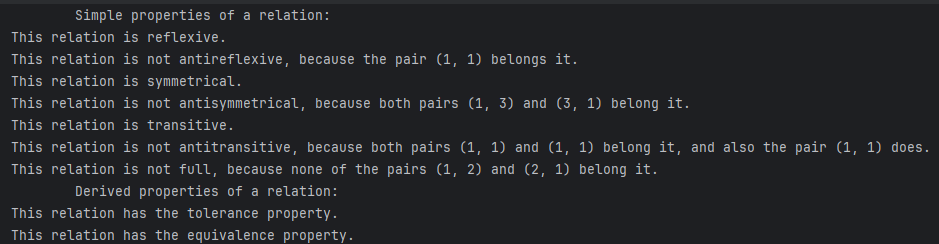
\includegraphics[width=180mm]{images/properties_output.png}
			\caption{Вывод сообщения о том, какими основными и производными свойствами обладает отношение $A$}
		}
	\end{figure}
	
	Самая важная информация, которую мы получили из этого ряда рассуждений --- отношение $A$ обладает свойством эквивалентности. Значит, мы можем перейти к поиску заданного им разбиения на классы эквивалентности.

	\section{Задание 3}
	\label{task3}

	{\bf Текст задания:} 3. Найти разбиение $\Phi$, определяемое заданным отношением эквивалентности.
	
	Выделим классы эквивалентности $[x]$ для каждого элемента $x \in M$.
	
	$[1] = \{1, 3, 5, 7, 9\}$ (поскольку $(1, 1) \in A$; $(3, 1) \in A$; $(5, 1) \in A$; $(7, 1) \in A$; $(9, 1) \in A$);
	
	$[2] = \{2, 4, 6, 8, 10\}$ (поскольку $(2, 2) \in A$; $(4, 2) \in A$; $(6, 2) \in A$; $(8, 2) \in A$; $(10, 2) \in A$).
	
	Поскольку в класс эквивалентности $[1]$ входят элементы 3, 5, 7, 9,  а в класс эквивалентности $[2]$ --- элементы 4, 6, 8, 10, это значит, что соответствующие пары входят в отношение $A$ (см. <<поскольку>> выше). Если пара $(x, y)$ входит в отношение, то классы эквивалентности $[x]$ и $[y]$ равны. Это можно доказать следующим образом: предположим, что они не равны. Тогда существует некоторый элемент $z$, причем либо $(z \in [x]) \& (z \notin [y])$, либо $(z \notin [x]) \& (z\in [y])$. 
	
	Рассмотрим первый случай. Для него истинно, что $((z, x) \in A) \& ((z, y) \notin A)$. Учитывая, что пара $(x, y) \in A$ по определению, можем воспользоваться свойством транзитивности отношения $A$: если $(z, x) \in A$ и $(x, y) \in A$, то справедливо $(z, y) \in A$. Получили противоречие.
	
	Аналогично для второго случая, $((z, x) \notin A) \& ((z, y) \in A)$. Пользуясь свойством симметричности отношения $A$, можем сказать, что если $(z, y) \in A$, то также истинно $(y, z) \in A$. Тем временем $((x, y) \in A)$ по умолчанию, и по свойству транзитивности, если $((x, y) \in A)$ и $(y, z) \in A$, то $(x, z) \in A)$. Снова получаем противоречие.
	
	В конечном итоге мы можем сделать вывод: если $((x, y) \in A)$ , то $[x]$ = $[y]$, и, соответственно, если $y \in [x]$, то $(y, x) \in A$ и $[x]$ = $[y]$. Значит, $[1]$ = $[3]$ = $[5]$ = $[7]$ = $[9]$ = $\{1, 3, 5, 7, 9\}$, и $[2]$ = $[4]$ = $[6]$ = $[8]$ = $[10]$ = $\{2, 4, 6, 8, 10\}$.
	
	Таким образом, разбиение $\Phi$, определяемое заданным отношением эквивалентности (то есть фактормножество отношения $A$) будет иметь вид $\Phi = \{\{1, 3, 5, 7, 9\}, \{2, 4, 6, 8, 10\} \}$.
	\section{Задание 4}
	\label{task4}

	{\bf Текст задания:} Написать программу, которая формирует разбиение, определяемое заданным отношением эквивалентности. 
	
	Для более удобной работы с разбиениями определим структуру, которая будет их хранить. Разбиение некоторого множества $M$ --- это множество попарно непересекающихся множеств, все элементы которых принадлежат множеству $M$, и эти множества при объединении дают исходное множество $M$. То есть каждый элемент множества M принадлежит ровно одному из множеств --- элементов разбиения, а потому организовать хранение можно таким образом: для каждого элемента множества $M$ хранить номер того элемента разбиения, которому он принадлежит. Для этого подойдет массив размера $|M|$, на i-той позиции которого хранится номер множества --- элемента разбиения, в которое входит элемент i (описание дано без учета того, что индексы в массиве нумеруются с 0, а множество содержит элементы, начиная с 1). Итого структуре splitting, реализующая разбиение, достаточно иметь два поля: 1) указатель на массив display, хранящий на каждой позиции i номер элемента разбиения, которому принадлежит принадлежит элементы исходного множества i, 2) мощность исходного множества max\_value. 
	
	Сразу же определим две базовые функции для разбиение: создание структуры и вывод содержимого на экран. При создании структуры нужно задать единственный вводный параметр: мощность множества, разбиение которого будет храниться, обозначаемая max\_value. Тогда выделяется память для хранения массива целых чисел длины max\_value, и все его элементы инициализируются нулями. Созданная структура в поле display будет хранить указатель на массив нулей, а в поле max\_value --- одноименный входной параметр. При печати используется следующий алгоритм: сначала производится проход по массиву display, в ходе которого находится максимальный номер множества --- элемента разбиения, max\_set. Затем в теле цикла for перебираются номера таких множеств от 1 до max\_set, и для каждого номера совершается проход по массиву display. Если на некоторой его позиции хранится текущий номер, значит, соответствующий элемент исходного множества входит в множество --- элемент разбиения. Этот элемент выводится на экран. До прохода по массиву выводится открывающая скобка <<\{>>, после прохода по массиву --- закрывающая <<\}>>, для обособления отдельных множеств --- элементов разбиения. Также скобки выводятся перед основной частью алгоритма и после нее, чтобы обозначить, что само разбиение --- тоже множество.
	
	\lstinputlisting[linerange={1-35}]{factor_sets/factor_sets.c} 
	
	Перейдем к основной части задания: написанию функции, которая по отношению эквивалентности $A$ формирует заданное ей разбиение или, говоря более точно, фактормножество по эквивалентности $A$. Вначале создается пустое разбиение с мощностью исходного множества той же, что и мощность множества, на котором построено отношение $A$. Также вначале инициализируется значением 1 переменная, отражающая номер classes\_amount текущего множества --- элемента разбиения, такие множества будет обозначать как $S_k$. Затем перебираются все элементы исходного множества --- обозначим текущий такой элемент как cur\_x. Если для cur\_x еще не определен номер classes\_amount множества $S_k$, к которому он относится, то еще одним перебором элементов исходного множества (обозначим текущий элемент вложенного перебора как cur\_y) формируется класс эквивалентности для текущего элемента. То есть, если пара (cur\_y, cur\_x) входит в отношение $A$, то cur\_y включается в текущее $S_k$, иначе говоря, в массиве display элементу под индексом cur\_y - 1 присваивается текущее classes\_amount. После перебора всех возможных cur\_y classes\_amount увеличивается на 1. В конечном итоге функция возвращает полученное разбиение.
		
	\lstinputlisting[linerange={37-51}]{factor_sets/factor_sets.c} 
	
	Наконец, в теле функции main создадим и заполним парами, в соответствии с заданным условием, отношение $A$. Создадим разбиение Phi и присвоим ему значение функции getFactorSet для отношения $A$, а потом выведем разбиение Phi на экран.
	
	\lstinputlisting[linerange={53-64}]{factor_sets/factor_sets.c} 
	
	\begin{figure}[h]
		\noindent\centering{
			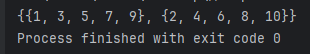
\includegraphics[width=90mm]{images/splitting_output.png}
			\caption{Вывод разбиения, определяемого отношением эквивалентности $A$}
		}
	\end{figure}
	
	Результаты выполнения программы для множества $A$ сошлись с полученными в ходе самостоятельных рассуждений в задании 3.
	
	
	\section{Вывод}
	\label{final}
	
	Если некоторое отношение обладает свойством эквивалентности, появляется возможность рассматривать более сложные его особенности и характеристики. Одной из таких характеристик является его фактормножество --- разбиение множества $M$, на котором построено отношение эквивалентности $A$, на классы эквивалентности. Класс эквивалентности для определенного элемента $x$ --- множество всех элементов $y$ таких, что $(y, x) \in A$. Классы эквивалентности обладают рядом свойств: для каждого элемента множества $M$ они не пустые; они равны, если в отношение $A$ входит пара из элементов, по которым они построены, и наоборот, не пересекаются, если соответствующая пара в отношение не входит, то есть $(x, y) \in A \to [x] = [y]$ и $(x, y) \notin A \to [x] \cap [y] = \emptyset$. В ходе лабораторной работы научились строить как отдельные классы эквивалентности, так и фактормножества вручную, а также написали программу для автоматического построения фактормножеств заданного множества по заданной эквивалентности.

\end{document}